\documentclass{article}

%% Page Margins %%
\usepackage{geometry}
\geometry{
    top = 0.75in,
    bottom = 0.75in,
    right = 0.75in,
    left = 0.75in,
}

\usepackage{amsmath}
\usepackage{graphicx}
\graphicspath{{report-assets/}}
\usepackage{parskip}
\usepackage{float}

\title{Assembly Project: Magical Drop}
\author{Norah Liu \and Tony Lin}

\begin{document}
\maketitle

\section{Instruction and Summary}

\begin{enumerate}

    \item Which milestones were implemented?

    DEMO 1:

    Milestone 1: A bordered $7\times14$ playing field with five starting rows of randomly coloured bubbles. Four colours are used, and the player is drawn below the board.

    Milestone 2: A/D movement, S grabbing of consecutive same-coloured bubbles, a held-bubble display, and row advancement every ten gameplay keypresses. The screen updates after actions, Q exits, and reaching the bottom row ends the game.

    Milestone 3: Boundary checks keep the player within columns 0--6. W places the held stack beneath the lowest bubble in the selected column, then checks for vertical matches of three or more and removes them. Remaining bubbles compact upward within their columns, and matching repeats after gravity until no new vertical match appears, producing chain reactions.


    \item How to view the game:

    \begin{enumerate}
    \item Open magicaldrop.asm
    \item Choose Bitmap. Set both the display width and height to 256 pixels, and both unit sizes to 8 pixels. Set the base address to \texttt{0x10008000}.
    \item Press Play to run the game, then click inside the bitmap so it receives keyboard input. Use lowercase letters for the controls.
    \end{enumerate}

    The bitmap has $32\times32$ drawing units. Each bubble takes up $2\times2$ units, or $16\times16$ pixels. The player appears below the board, and the squares on the right show the bubbles being held.

\begin{figure}[ht!]
    \centering
    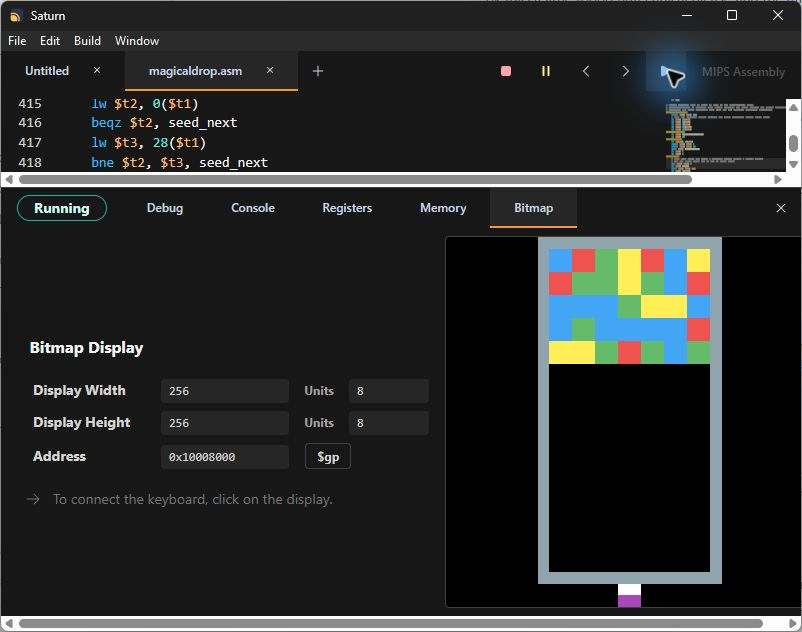
\includegraphics[width=0.4\textwidth]{game-scene.png}
    \label{Instructions}
\end{figure}



\item Game Summary:
\begin{itemize}
\item \textbf{Rearrange bubbles to keep the board from filling up.}\\
Player collects bubbles from one column and throws them into another to form vertical matches. New rows gradually push the board downward, so clearing bubbles creates room to keep playing.

\item \textbf{Movement, grabbing, and throwing use A/D, S, and W.}\\
Player moves one column at a time and stops at either edge. Grabbing searches upward for the lowest bubble, then collects the consecutive stack of that colour. The held stack is stored as a colour and a count, so only that colour can be collected until the stack is thrown. Q exits the program.

\item \textbf{Matching clears vertical runs of three or more.}\\
After a throw, the program scans for three equal, nonzero cells in a column. It marks matches in \texttt{bubbles\_to\_clear} before deleting them, allowing overlapping triples in a longer run to clear together. Then each column is compacted upward, preserving the order of its remaining bubbles. The program scans again after gravity and repeats the clear-and-rise process until no vertical match remains, producing chain reactions. Horizontal neighbours do not clear unless they form part of their own vertical match; horizontal flood fill is not implemented.

\item \textbf{Every ten gameplay keypresses advances the board.}\\
A, D, S, and W increase the key counter. When the counter is at ten, the counter resets, existing rows shift down, and seven random bubbles fill the top row. Rows are copied from bottom to top to avoid overwriting cells before they are moved. Waiting without input does not advance the board.

\item \textbf{The game ends when a bubble reaches the bottom row.}\\
After an action and any row advancement, the program checks all seven cells in row 13. A nonempty cell sets the game-over flag. A throw that would exceed the column's capacity also ends the game. The final board is drawn before execution stops. 

\item \textbf{The board and matching data are stored separately from the display.}\\
The \texttt{board} array contains 98 four-byte words, using 392 bytes. Zero means empty; 1--4 represent red, blue, yellow, and green. Cells are stored row by row, so cell $(r,c)$ is at \texttt{board} $+4(7r+c)$, with rows 0--13 and columns 0--6. The matching array uses another 392 bytes. Separate words store the player column, held colour and count, key counter, and game-over flag; the palette holds five colour words.

\item \textbf{Drawing converts the stored board into coloured rectangles.}\\
The drawing routine looks up each cell's colour in the palette and writes it to bitmap memory. The display begins at \texttt{0x10008000}, uses 4096 bytes, and stores drawing unit $(x,y)$ at \texttt{0x10008000} $+4(32y+x)$. Each board cell is drawn as a $2\times2$ rectangle. The player and held-bubble indicators are erased and redrawn to reflect their current state.

\begin{figure}[H]
    \centering
    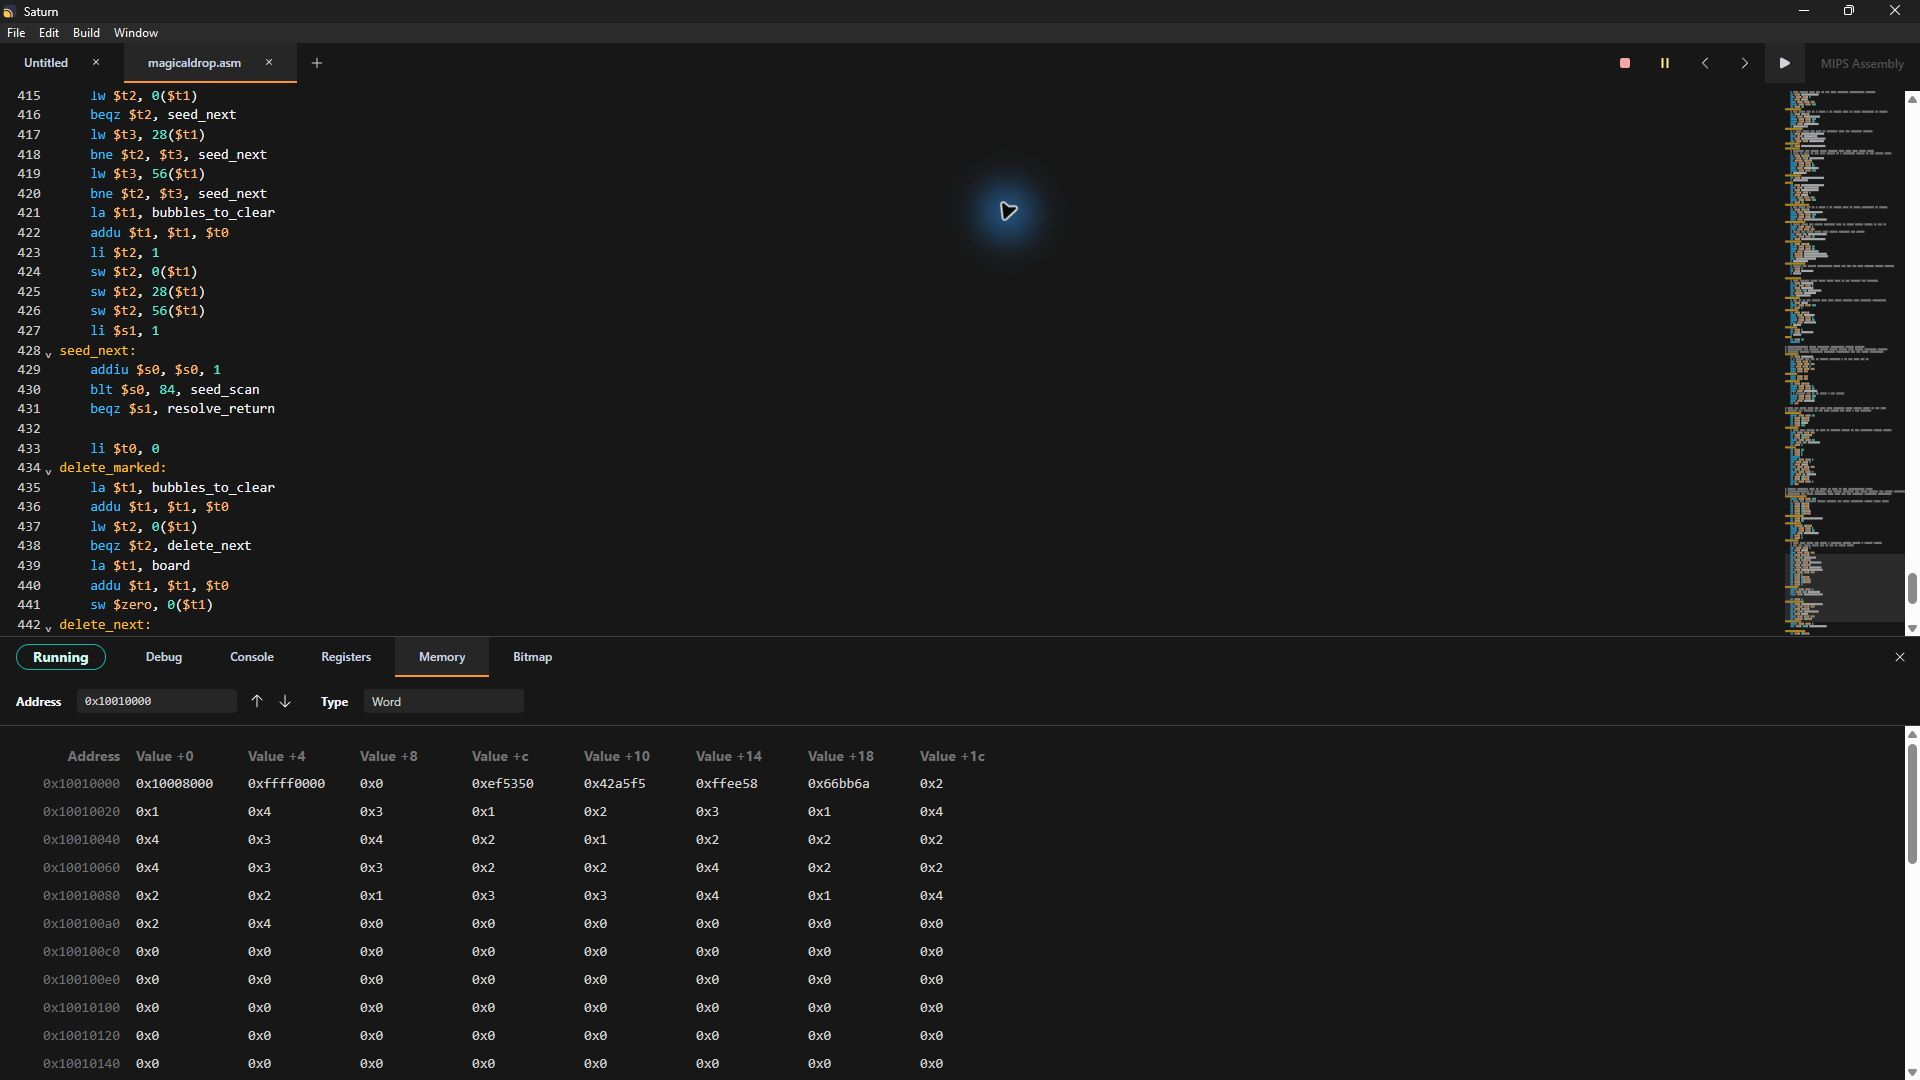
\includegraphics[width=0.85\textwidth]{memory-board.png}

    \vspace{0.2cm}

    \IfFileExists{memory-variables.png}{\includegraphics[width=0.85\textwidth]{memory-variables.png}}{}

    \label{Memory}
\end{figure}

\item \textbf{The main loop connects keyboard input to changes on screen.}\\
The program briefly sleeps, checks keyboard status at \texttt{0xFFFF0000}, and reads the character at \texttt{0xFFFF0004}. It runs the selected action, updates the key counter, checks for a loss, and redraws as needed. The short sleep limits input polling.


\end{itemize}

\end{enumerate}

\section{Attribution Table}

\begin{center}
\begin{tabular}{|| c | c ||}
\hline
 Norah Liu (student number: TBD) & Tony Lin (student number: TBD) \\
\hline
\shortstack{Board initialization and drawing\\[2pt]
{\footnotesize\texttt{main, clear\_board, random\_bubbles}}\\
{\footnotesize\texttt{draw\_cells, draw\_rect}}}
&
\shortstack{Player movement and keyboard input\\[2pt]
{\footnotesize\texttt{poll\_keyboard, handle\_key}}\\
{\footnotesize\texttt{move\_left, move\_right}}}\\[5pt]
\hline
\shortstack{Displaying the held bubbles\\[2pt]
{\footnotesize\texttt{redraw, draw\_held, draw\_rect}}}
&
\shortstack{Bubble grabbing and throwing\\[2pt]
{\footnotesize\texttt{grab, find\_bottom, found\_bottom}}\\
{\footnotesize\texttt{grab\_chain, finish\_grab, throw}}}\\[5pt]
\hline
\shortstack{Vertical matching, gravity and chains\\[2pt]
{\footnotesize\texttt{resolve\_matches, clear\_marks}}\\
{\footnotesize\texttt{seed\_scan, delete\_marked}}}
&
\shortstack{Throw placement and capacity checks\\[2pt]
{\footnotesize\texttt{throw\_find\_bottom, throw\_position}}\\
{\footnotesize\texttt{throw\_place, throw\_overflow}}}\\[5pt]
\hline
\shortstack{Keystroke-based row advancement\\[2pt]
{\footnotesize\texttt{action\_done, advance\_row}}\\
{\footnotesize\texttt{shift\_row, new\_row}}}
&
\shortstack{Checking boundaries and game over\\[2pt]
{\footnotesize\texttt{move\_left, move\_right, check\_loss}}\\
{\footnotesize\texttt{loss\_scan, set\_loss}}\\
{\footnotesize\texttt{finish\_frame, quit}}}\\[5pt]
\hline
\shortstack{Half of report and demo preparation\\[2pt]
{\footnotesize Whole-program review}}
&
\shortstack{Half of report and demo preparation\\[2pt]
{\footnotesize Whole-program review}}\\[5pt]
\hline
\end{tabular}
\end{center}

\end{document}

